% !TEX encoding = UTF-8 Unicode
\documentclass[12pt]{article}
\usepackage[T2A]{fontenc}
\usepackage[utf8]{inputenc}
\usepackage[english, russian]{babel}

\usepackage{graphicx}
\graphicspath{{images/}}
\usepackage{amsmath, amsthm, amssymb, thmtools}
\usepackage{cite}

\usepackage{geometry}
\usepackage{indentfirst}
\textheight = 24cm
\textwidth = 16cm
\oddsidemargin = 0cm
\topmargin = -1.5cm
\parindent = 24pt
\parskip = 0pt
\flushbottom
\linespread{1.3}

\declaretheorem[style = definition, name = Определение]{definition}

\begin{document}
\begin{titlepage}
\begin{center}

	Московский государственный университет имени~М.~В.~Ломоносова

	\bigskip

	\includegraphics[width=50mm]{msu.eps}
	
	\bigskip

	Факультет Вычислительной Математики и Кибернетики\\
	Кафедра Математических Методов Прогнозирования\\[10mm]

	\textsf{\large\bfseries
		ВЫПУСКНАЯ КВАЛИФИКАЦИОННАЯ РАБОТА\\[10mm]
		<<Слияние перекрывающихся триангуляций Делоне на основе минимальных остовных деревьев>>
	}\\[10mm]
	
	\begin{flushright}
		\parbox{0.5\textwidth}{
		Выполнила:\\
		студентка 4 курса 417 группы\\
		\emph{Готман Мария Леонидовна}\\[5mm]	
		Научный руководитель:\\
		д.т.н., профессор\\
		\emph{Местецкий Леонид Моисеевич}\\[5mm]
		}
	\end{flushright}

	\vspace{\fill}
	Москва, 2015
\end{center}
\end{titlepage}

\newpage

\tableofcontents

\newpage
\begin{abstract}

\end{abstract}

\newpage
\section{Введение}

\section{Терминология и постановка задачи}

\subsection{Основные определения}
Пусть на евклидовой плоскости задано $\textbf{S}$ --- множество из не менее трех точек, не все из которых лежат на одной прямой.
Используя  \cite[стр.~7-8]{Skvortsov}, \cite{MestOverlap} введем ряд ключевых определений которые понадобятся нам для дальнейшего понимания задачи.

Точки, входящие во множество $\textbf{S}$ будем называть {\itshape сайтами}.
{\itshape Триангуляцией} конечного множества точек $\textbf{S}$ называется планарный граф с вершинами из $\textbf{S}$,
все внутренние области которого являются треугольниками.
Триангуляция называется {\itshape выпуклой}, если минимальный многоугольник, охватывающий все ее треугольники, будет выпуклым.
Далее под термином {\itshape грань} будем понимать только конечную треугольную грань триангуляции.
Ребро и грань называются {\itshape инцидентными}, если они имеют две общие вершины.
Ребра, инцидентные одной грани, называются {\itshape смежными}.
Ребро, имеющее менее двух инцидентных граней, называется {\itshape открытым}.

Окружность называется {\itshape пустой}, если она не содержит внутри себя сайтов.
Прямая линия, по одну сторону от которой нет сайтов, называется {\itshape несобственной} пустой окружностью.
Окружность, проходящая через сайт, называется {\itshape инцидентной} этому сайту.
{\itshape Ребром Делоне} называется ребро, инцидентные сайты которого имеют общую пустую инцидентную окружность.
{\itshape Гранью Делоне} называют грань, вершины которой имеют общую пустую инцидентную окружность.

Дадим два эквивалентных определения:

\begin{definition}
{\itshape Триангуляцией Делоне (ТД) $Del(\textbf{S})$} множества точек $\textbf{S}$ называется выпуклая триангуляция,
у которой описанная окружность каждой треугольной грани является пустой,
т.е. все грани которой являются гранями Делоне.
\end{definition}

\begin{definition}
{\itshape Триангуляцией Делоне} множества точек $\textbf{S}$ называется выпуклая триангуляция,
у которой для каждого ребра существует пустая инцидентная сайтам-вершинам окружность,
т.е. все ребра которой являются ребрами Делоне.
\end{definition}

{\itshape Пучком} сайта $p \in \textbf{S}$ называют множество ребер триангуляции, инцидентных сайту $p$.
Пучок сайтов будем представлять в виде двунаправленного циклического списка сайтов $p_1, \ldots, p_k$,
смежных с $p$ в триангуляции, так чтобы они шли в направлении обхода против часовой стрелки относительно $p$.

\subsection{Постановка задачи}
Задача слияния двух перекрывающихся триангуляций Делоне ставится следующим образом.
Даны два конечных линейно неразделимых множества сайтов $\textbf{B}$ и $\textbf{W}$ (допускается их полное перемешивание),
а также их триангуляции Делоне $Del(\textbf{B})$ и $Del(\textbf{W})$.
Нужно построить триангуляцию Делоне на объединенном множестве сайтов $Del(\textbf{B} \cup \textbf{W})$.

Будем считать, что сайты раскрашены в два цвета: множество черных сайтов $\textbf{B}$ и множество белых сайтов $\textbf{W}$.
Триангуляции множеств $\textbf{B}$ и $\textbf{W}$ будем называть исходными,
искомую триангуляцию $Del(\textbf{B} \cup \textbf{W})$ будем называть объединенной.
Пример исходных данных и искомой триангуляции приведен на рис. \ref{pic:model_data}.

\begin{figure}[htb!]
	\begin{minipage}[h]{0.49\linewidth}
		\center{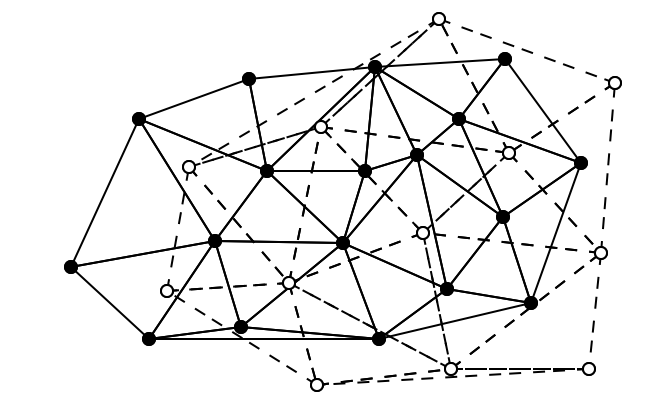
\includegraphics[width=1\linewidth]{model_data.png}}
	\end{minipage}
	\hfill
	\begin{minipage}[h]{0.49\linewidth}
		\center{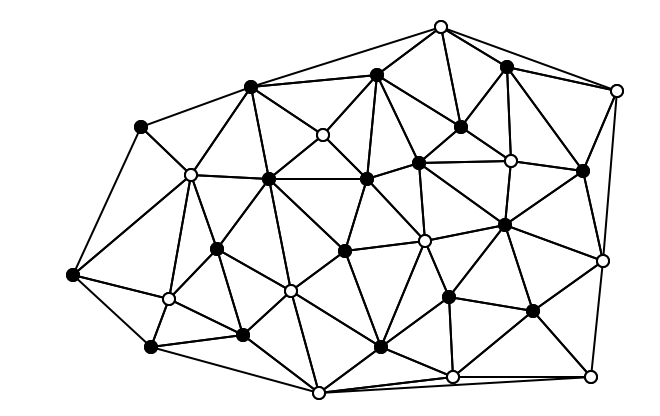
\includegraphics[width=1\linewidth]{model_res.png}}
	\end{minipage}
	\caption{Исходные триангуляции и объединенная триангуляция}
	\label{pic:model_data}
\end{figure}

\section{Описание алгоритма}
В данном разделе введем основные понятия, связанные с разрушением ребер в исходных триангуляциях
и построением новых ребер объединенной триангуляции,
а также дадим общую схему алгоритма слияния перекрывающихся триангуляций Делоне \cite{MestOverlap}.

В объединенной триангуляции Делоне $Del(\textbf{B} \cup \textbf{W})$ существуют ребра двух типов:
одноцветные, которые были взяты из исходных триангуляций, и разноцветные, сайты-вершины которых взяты из разных исходных триангуляций.

Множество вершин и ребер (ребер и граней) называется {\itshape связным}, если для любой пары элементов этого множества
существует цепь из попарно инцидентных вершин и ребер (ребер и граней), принадлежащих этому множеству.

В объединенной триангуляции существуют максимальные связные одноцветные подмножества вершин и ребер,
переходящие без изменений из исходных триангуляций, которые будем называть {\itshape лоскутами}.
Ребра и грани, не вошедшие в лоскуты, должны быть разрушены.
Такие связные подмножества будем называть {\itshape разрезами}.
При построении разрезов будут удалены некоторые грани, что приведет к образованию открытых ребер.
Связную цепочку вершин и открытых ребер, состоящих из ребер одного цвета, будем называть {\itshape краем}.
Максимальные связные подмножества разноцветных ребер и граней объединенной триангуляции будем называть {\itshape швами}.
Разноцветные ребра будем называть {\itshape стежками}.

При данных определениях построение объединенной триангуляции Делоне состоит из нескольких частей: построения разрезов,
выделения лоскутов исходных триангуляций и построения швов.
Каждый шов соединяет два разноцветных края, образованных после разрушения ребер, вошедших в разрезы.
В начале работы алгоритма краями исходных триангуляций являются их выпуклые оболочки.
По мере построения разрезов и швов количество краев меняется
(увеличивается при построении разрезов и уменьшается при построении швов).
В объединенной триангуляции остается только один край --- граница выпуклой оболочки.

{\itshape Стартером} будем называть пару разноцветных сайтов, образующих ребро Делоне,
еще не включенное в объединенную триангуляцию.
Стартер нужен для запуска процесса построения разреза и шва.
Построение смежных стежков для стартера можно вести по разные стороны от него.
Для определенности будем полагать, что стартер имеет левый и правый сайты,
построение стежка происходит в направлении перед стартером.
На рис. \ref{pic:dir} черным цветом обозначен стартер, зеленым новый стежок, построенный в направлении перед стартером.

\begin{figure}[htb!]
	\center{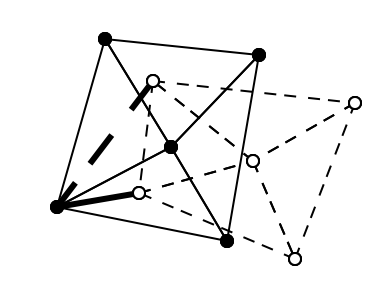
\includegraphics[width=0.5\linewidth]{direct_starter.png}}
	\caption{Построение новых стежков}
	\label{pic:dir}
\end{figure}

Шов может быть двух типов.
{\itshape Разомкнутым} швом называется шов, имеющий два стежка, принадлежащих выпуклой оболочке объединенной триангуляции,
то есть принадлежащих граничным ребрам $Del(\textbf{B} \cup \textbf{W})$.
{\itshape Циклическим} называется шов, имеющий только внутренние ребра объединенной триангуляции.

В процессе построения разомкнутого шва сначала находим одну его часть,
затем продолжаем движение по другую сторону стартера и находим оставшуюся часть разреза.
В циклическом шве в некоторый момент времени стартер совпадет с новым стежком,
на этом построение шва будет закончено.

Введем понятие минимального остовного дерева.
{\itshape Минимальным остовным деревом (МОД)} триангуляции Делоне называется ее связный подграф,
имеющий наименьшую суммарную длину ребер.
Пусть на плоскости задано $N$ точек.
{\itshape Евклидовым МОД} называется связный подграф, вершинами которого являются все $N$ точек, суммарная длина всех ребер которого минимальна.
Известно, что МОД ТД является евклидовым минимальным остовным деревом для множества сайтов ТД \cite[стр. 229, 277]{Preparata}.
МОД исходных триангуляций Делоне понадобятся в процессе построения стартеров.


\subsection{Общая схема алгоритма}
\begin{enumerate}
	\item Построить минимальные остовные деревья для обеих исходных триангуляций.
	\item Построить начальный стартер
	\item \label{alg1:l1} Построить разрез и шов
	\begin{enumerate}
		\item Объявить стартер текущим стежком
		\item Провести коррекцию одноцветных ребер (построение разреза)
		\item \label{alg1:l2} Построить новый стежок
		\item Если построить новый стежок не удалось, развернуть стартер и перейти к пункту \ref{alg1:l1}
		\item Если построить новый стежок не удалось во второй раз, закончить построение шва
		\item Удалить ребра, пересекающих новую грань
		\item Проверить совпадение со стартером, в случае совпадения закончить построение шва, иначе перейти к шагу \ref{alg1:l2}
	\end{enumerate}
	\item Поиск очередного стартера
	\item Если стартер найден, перейти к пункту \ref{alg1:l1}, иначе закончить работу алгоритма
\end{enumerate}

\subsection{Выбор структуры данных}

\subsection{Построение разрезов и швов триангуляций Делоне}

\subsection{Поиск стартеров}

\subsubsection{Поиск первого стартера}

\subsubsection{Минимальные остовные деревья}

\subsubsection{Поиск последующих стартеров}

\section{Оценка вычислительной сложности алгоритма}

\section{Эксперименты}

\subsection{Программная реализация}

\subsection{Вычислительные эксперименты}

\section{Заключение}

\newpage

\addcontentsline{toc}{section}{Использованная литература}

\bibliographystyle{utf8gost705u}
\bibliography{report_diploma}
\end{document}